\documentclass{article}
\usepackage[T1]{fontenc}
\usepackage{lmodern}
\usepackage{graphicx}
\usepackage{amsmath,amssymb}
\usepackage[a4paper,margin=2cm]{geometry}
\usepackage[absolute,overlay]{textpos}
\setlength{\TPHorizModule}{1mm}
\setlength{\TPVertModule}{1mm}
\usepackage[indonesian]{babel}
\usepackage{hyperref}
\setlength{\emergencystretch}{2em}
% unit: Halaman 47

\begin{document}

% === Halaman 47 (llm) ===

\section*{Kriptologi}

\vspace{166.91mm}

Kriptologi (\textit{cryptology}): studi mengenai kriptografi dan kriptanalisis.

\vspace{50mm}

% deskripsi: Diagram hierarki yang menunjukkan Kriptologi terbagi menjadi dua cabang utama: Kriptografi (ilmu dan seni untuk menjaga keamanan pesan) dan Kriptanalisis (ilmu dan seni untuk memecahkan cipherteks), dengan panah dua arah yang menghubungkan keduanya.
% bbox normalisasi: [0.1870, 0.3680, 0.7860, 0.9300]
\begin{textblock*}{125.79mm}(39.27mm,109.30mm)
\noindent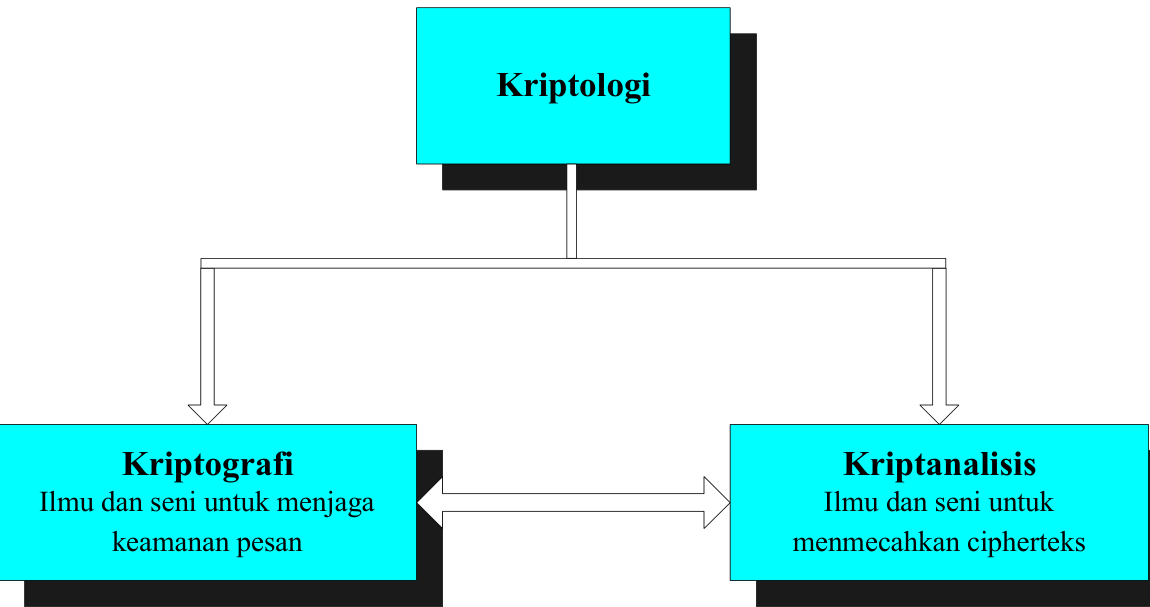
\includegraphics[width=125.79mm,height=166.91mm]{../../images/llm/page_047_img_01.png}%
\end{textblock*}

\end{document}
